\begin{frame}{some bad history}
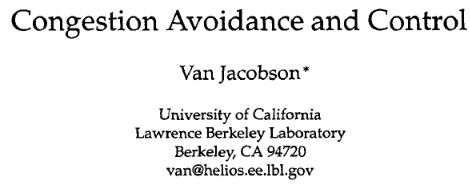
\includegraphics[width=0.6\textwidth]{../congest/jacobson-title}
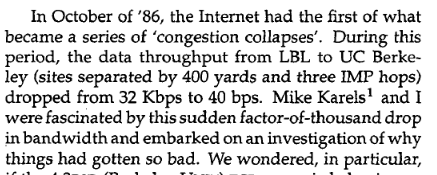
\includegraphics[width=0.6\textwidth]{../congest/jacobson-disaster}
\end{frame}

\begin{frame}{the overloaded switch}
\begin{itemize}
\item let's say switch can handle 50 packets/second
\item but has:
    \begin{itemize}
    \item 100 packets/second from test flow sending as fast as it can
    \item 10 packets/second from other session
    \end{itemize}
\item expected \textit{loss rate} (\% packets lost)?
\item expected \% test flow packets lost?
\item expected other session packets lost?
\end{itemize}
\end{frame}

\begin{frame}{modeling who gets dropped}
    \begin{itemize}
    \item it kinda does matter\ldots
    \item sending in big bursts or spread out (``pacing'')?
        \begin{itemize}
        \item bursts can overload queues even though average rate is low
        \end{itemize}
    \item how switch's queue works?
        \begin{itemize}
        \item queue size (handling bursts), way to choose what to drop
        \end{itemize}
    \item random or fixed intervals between sending?
    \vspace{.5cm}
    \item<2-> but we'll \myemph<2>{simplify}, assuming---
        \begin{itemize}
        \item a flow's arrivals are randomly spaced
        \item drops hit packets at random
        \item queue is ``pretty big''
        \end{itemize}
    \end{itemize}
\end{frame}

\begin{frame}{the overloaded switch}
\begin{itemize}
\item let's say switch can handle 50 packets/second
\item but has:
    \begin{itemize}
    \item 100 packets/second from test flow (checking window size) 
    \item 20 packets/second from other session
    \end{itemize}
\item expected \textit{loss rate} (\% packets lost)? $\frac{100+20-50}{100+20}=58\%$
\item expected \% test flow packets lost? $58\%$
\item expected \% other session packets lost? $58\%$
\item<2-> \myemph{\ldots but I missed something}
\end{itemize}
\end{frame}

\begin{frame}{a virtuous cycle}
\begin{itemize}
\item what is other session going to when 58\% of its packets are lost?
    \begin{itemize}
    \item probably resend them
    \end{itemize}
\item what about when resent packets are lost?
    \begin{itemize}
    \item probably resent again
    \end{itemize}
\vspace{.5cm}
\item if other session doesn't slow down, then\ldots
\item $10$ pkt/s $\rightarrow10+58\%\cdot10+58\%^2\cdot10 \ldots\approx 48$ pkt/s
\end{itemize}
\end{frame}


\begin{frame}{the overloaded switch (revised)}
\begin{itemize}
\item let's say switch can handle 50 packets/second
\item but has:
    \begin{itemize}
    \item 100 packets/second from test flow (checking window size) 
    \item 20 packets/second from other session $\rightarrow 48$ with resends
    \end{itemize}
\item expected \textit{loss rate} (\% packets lost)? $\frac{100+48-50}{100+48}=66\%$
\item expected \% test flow packets lost? $66\%$
\item expected \% other session packets lost? $66\%$
    \begin{itemize}
    \item<2-> means that 48 pkt/sec is slight underestimate
    \item<2-> though realistically other session should slow down
    \end{itemize}
\end{itemize}
\end{frame}

\begin{frame}{aside: latency (1)}
\begin{itemize}
\item 58\% packet loss $\rightarrow$ average packet sent 2.4 times
\item need one round-trip time (RTT) to detect loss
    \begin{itemize}
    \item probably from duplicate ACK
    \item if detecting via timeout, probably longer
    \end{itemize}
\item so need 1.4 RTTs (detecting loss 1.4 times) extra time 
\item mean latency $= \frac{1.4 \text{RTTs}}{0.5 \text{RTTs}}$ times normal $= 2.8$ times normal
\end{itemize}
\end{frame}

\begin{frame}{aside: high-percentile latency}
\begin{itemize}
\item 58\% packet loss
\item about 10\% of time need more than 4 retransmissions
\item about 5\% of the time need more than 5 retransmissions
\item about 1\% of the time need more than 8 retransmissions
\end{itemize}
\end{frame}

\begin{frame}{sliding windows and retransmissions}
    \begin{itemize}
    \item assuming that other session doesn't slow down
    \vspace{.5cm}
    \item sliding window approach slows down on losses
    \end{itemize}
\end{frame}

\begin{frame}{sliding window throughput collapse}
\begin{itemize}
\item let's say doing sliding window with 100 packet window
\item if 1\% of the time, we need to resend a packet 8 times, then
\item probably need around 8 RTTs to send all 100 packets in window
\vspace{.5cm}
\item<2-> $\approx$ 8 times slower with same window size
\end{itemize}
\end{frame}

\begin{frame}{performance v load}
\begin{tikzpicture}

\end{tikzpicture}
\end{frame}
